\documentclass[hyphens,aspectratio=169,dvipsnames]{beamer}
\usepackage{graphicx}
\usepackage{xcolor}
\usepackage{amssymb}
\usepackage{amsmath}
\usepackage{mathtools}
\usepackage{textcomp}
\usepackage{moresize}
\usepackage{framed}
\usepackage{minted}
\usepackage{relsize}
\usepackage{tikz}
\usepackage{comment}
\usetikzlibrary{shapes.geometric, arrows, positioning}
\usetheme{Berlin}
\usecolortheme[RGB={0,95,47}]{structure}
\beamertemplatenavigationsymbolsempty

\makeatletter
\AtBeginEnvironment{minted}{\dontdofcolorbox}
\def\dontdofcolorbox{\renewcommand\fcolorbox[4][]{##4}}
\makeatother

\newcommand{\textpf}[1]{\texttt{\color{black}\fcolorbox{lightgray}{lightgray}{#1}}}

\begin{document}

\begin{frame}[fragile]{Disclaimer}
    \begin{itemize}
        \pause \item This is a large, important lecture.
        \pause \item Please interrupt me as soon as something doesn't make sense.
        \pause \item I would legitimately rather not finish all of the material than have any of you not understand what's going on.
        \pause \item I will simplify some statements in this lecture for clarity. Later in this class (and in future classes), we'll pull back the curtain on some of these statements.
        \pause \item This lecture will require your complete attention :)
    \end{itemize}
\end{frame}

\begin{frame}[fragile]{Disclaimer 2}
    We will be using the X-Hour!!
\end{frame}

\begin{frame}[fragile]{Disclaimer 3}
    Assignment 1 goes out today!
\end{frame}

\begin{frame}[fragile]{Memory}
    \begin{itemize}
        \pause \item Computers have many kinds of ``memory."
        \begin{itemize}
            \pause \item Disk (slow)
            \pause \item RAM (medium)
            \pause \item Cache (fast)
            \pause \item Registers (fastest)
        \end{itemize}
        \pause \item Usually, when a computer scientist says ``memory," they mean RAM.
    \end{itemize}
\end{frame}

\begin{frame}[fragile]{RAM}
    \begin{itemize}
        \pause \item \textbf{Your computer's memory is a big array of bytes}.
        \pause \item If you have 16GB of RAM, then this array has $16 \cdot 2^{30}$ entries in it.
        \pause \item A \textbf{memory address} is simply an index into this big array.
    \end{itemize}
\end{frame}

\begin{frame}[fragile]{Executables}
    \begin{itemize}
        \pause \item Recall that when you compile a C program, the compiler spits out a file named \textpf{a.out} (by default).
        \pause \item What is contained within \textpf{a.out}?
            \begin{enumerate}
                \pause \item code
                \pause \item data (e.g., global variables)
                \pause \item metadata
            \end{enumerate}
    \end{itemize}
\end{frame}

\begin{frame}[fragile]{Executing Executables}
    \begin{itemize}
        \pause \item Recall that you run your C program by typing \textpf{./a.out} into the shell.
        \pause \item What does this actually do?
            \begin{enumerate}
                \pause \item Loads the \textbf{code and data} into the computer's memory at addresses specified by the metadata.
                \pause \item \textbf{Starts executing} from the code's entry point (which is specified in the metadata).
            \end{enumerate}
    \end{itemize}
\end{frame}

\begin{frame}[fragile]{What a CPU Does}
    \begin{enumerate}
        \pause \item Read a machine code instruction from memory.
        \pause \item Do what it says to do.
        \pause \item Read the next machine code instruction from memory.
        \pause \item ... \pause (forever)
    \end{enumerate}
\end{frame}

\begin{frame}[fragile]{Addresses}
    \begin{itemize}
        \pause \item In a running program (C or otherwise), all data and code exists in memory.
        \pause \item When you run \mintinline{c}{char x = 5;}, a byte in memory gets set to 5.
    \end{itemize}
\end{frame}

\begin{frame}[fragile]{Example}
    \begin{itemize}
        \pause \item Suppose that the address of \textpf{x} is \textpf{1234}.
        \pause \item Then, when we run \textpf{x = 5}, this happens:
    \end{itemize}

    \pause
    \begin{center}
    \begin{tabular}{| c | c | c | c | c | c |}
        \hline
        index & 0  & 1  & ... & 1234 & ... \\
        \hline
        value & ?? & ?? & ... & ??   & ... \\
        \hline
    \end{tabular}
    \end{center}
\end{frame}

\begin{frame}[fragile]{Example}
    \begin{itemize}
        \item Suppose that the address of \textpf{x} is \textpf{1234}.
        \item Then, when we run \textpf{x = 5}, this happens:
    \end{itemize}

    \begin{center}
    \begin{tabular}{| c | c | c | c | c | c |}
        \hline
        index & 0  & 1  & ... & 1234 & ... \\
        \hline
        value & ?? & ?? & ... & 5    & ... \\
        \hline
    \end{tabular}
    \end{center}
\end{frame}

\begin{frame}[fragile]{Arrays}
    C has arrays, just like Java.

    \pause Two important operations that C's arrays support are
    \begin{enumerate}
        \pause \item Unary \textpf{*}, a.k.a. dereference
            \begin{itemize}
                \pause \item Accesses the first item in the array.
            \end{itemize}
        \pause \item Binary \textpf{+} with integer operand
            \begin{itemize}
                \pause \item Takes the tail of the array.
                \pause \item For example, adding 1 to an array in C is similar to slicing a list in Python with \textpf{[1:]}.
            \end{itemize}
    \end{enumerate}
\end{frame}

\begin{frame}[fragile]{Declaring a Local Array}
    \begin{itemize}
        \pause \item The following program declares a local array of 5 \textpf{unsigned int}s named \textpf{ary}, and returns its first element.
            \inputminted{c}{uninitialized_local_array.c}
        \pause \item Q: What does this program return?
        \pause \item A: \textbf{It's UB.}
    \end{itemize}
\end{frame}

\begin{frame}[fragile]{Declaring a Global Array}
    \begin{itemize}
        \pause \item The following program declares a global array of 5 \textpf{unsigned int}s named \textpf{ary}, and returns its first element.
            \inputminted{c}{uninitialized_global_array.c}
        \pause \item Q: What does this program return?
        \pause \item A: \textbf{0. All global variables are default-initialized to 0.}
        \pause \item This is unintuitive! You'll understand the reason for this later in the course.
    \end{itemize}
\end{frame}

\begin{frame}[fragile]{VLAs}
    \begin{itemize}
        \pause \item The length of an array must be a compile-time constant expression.
        \pause \item On some compilers, this isn't enforced, so the following would work:
            \inputminted{c}{vla.c}
        \pause \item Arrays where the size is not a compile-time constant are known as ``variable-length arrays" (VLAs).
        \pause \item They are error-prone and difficult to reason about, and were removed from the C standard in 2011. Do not use them!
        \pause \item From now on, always compile with \textpf{-Wvla} so the compiler will warn you when you accidentally use a VLA.
    \end{itemize}
\end{frame}

\begin{frame}[fragile]{Initializing an Array}
    \begin{itemize}
        \item \pause Just like \textpf{struct}s, arrays can be initialized with intializer lists:
        \inputminted{c}{initialized_local_array.c}
    \end{itemize}
\end{frame}

\begin{frame}[fragile]{Default-Initializing an Array}
    \begin{itemize}
        \pause \item Initializer lists are permitted to have fewer elements than the length of the array.
            \inputminted{c}{default_initialized_local_array.c}
        \pause \item Q: What is the second element in the array?
        \pause \item A: \textbf{When an array (global or local) is assigned to an initializer list with less elements than the array's length, the remaining elements are default-initialized to 0.}
        \pause \item This is really unintuitive!
    \end{itemize}
\end{frame}

\begin{frame}[fragile]{Implicit Array Lengths}
    \begin{itemize}
        \pause \item Q: What is the length of the array in this program?
            \inputminted{c}{implicit_length_local_array.c}
        \pause \item A: \textbf{1, thankfully :)}
    \end{itemize}
\end{frame}

\begin{frame}[fragile]{Array Indexing}
    \begin{itemize}
        \item \pause To index an array for element \textpf{n},
            \begin{itemize}
                \pause \item Add \textpf{n} to the array.
                \pause \item Dereference the result.
            \end{itemize}
        \pause \item Q: What does this return?
            \inputminted{c}{manual_array_index.c}
    \end{itemize}
\end{frame}

\begin{frame}[fragile]{Array Indexing}
    \begin{itemize}
        \pause \item Q: What does this return?
            \inputminted{c}{manual_array_index_2.c}
    \end{itemize}
\end{frame}

\begin{frame}[fragile]{The \textpf{[]} Operator}
    \begin{itemize}
        \pause \item The \textpf{[]} operator combines the \textpf{*} and \textpf{+} operators.
        \pause \item That is, the following is equivalent to the programs on the previous two slides:
            \inputminted{c}{regular_array_index.c}
        \pause \item Q: Copy this program down and build it. How does it behave when you index the array for
        \begin{itemize}
            \pause \item -1?
            \pause \item 10?
            \pause \item -10?
            \pause \item 999999999?
        \end{itemize}
    \end{itemize}
\end{frame}

\begin{frame}[fragile]{Some Fun Trivia}
    \begin{itemize}
        \pause \item Suppose that \textpf{a} is an array and \textpf{i} is an integer.
        \pause \item Then, \textpf{a[i]} and \textpf{*(a + i)} are \textbf{exactly equivalent}.
        \pause \item Knowing this, what does the following program do?
            \inputminted{c}{weird_array_index.c}
    \end{itemize}
\end{frame}

\begin{frame}[fragile]{Arrays and \textpf{sizeof}}
    \begin{itemize}
        \pause \item Recall that the \textpf{sizeof} operator returns the number of bytes used to represent its argument.
        \pause \item Knowing this, how would you generically take the length of a nonempty array?
        \pause \item \textbf{Given an array \textpf{ary}, its length is}
        \begin{minted}{c}
            sizeof(ary)) / sizeof(ary[0])
        \end{minted}
    \pause \item Q: Try writing a function that takes as input an array of \textpf{unsigned int} and returns its length. Does it behave the way you expect?
    \end{itemize}
\end{frame}

\begin{frame}[fragile]{Activity: Arrays and \textpf{sizeof}}
    \begin{itemize}
        \pause \item Define a \textpf{struct} with 4 fields:
            \begin{itemize}
                \item 1 \textpf{int},
                \item 2 \textpf{char}s,
                \item 1 \textpf{long}.
            \end{itemize}
        \pause \item Make an array containing 3 of your \textpf{struct}s.
        \pause \item What do you expect the \textpf{sizeof} your array is?
        \pause \item Take its size using \textpf{sizeof}. Is it what you expect?
        \pause \item Now, take the \textpf{sizeof} your array \textpf{+ 1}. Is it what you expect?
        \pause \item Try reordering the fields in your \textpf{struct}. How does it affect the \textpf{sizeof} computations? Try to make sense of this :)
    \end{itemize}
\end{frame}

\begin{frame}[fragile]{Intro to Pointers}
    \begin{itemize}
        \pause \item Recall the following program:
            \inputminted{c}{uninitialized_local_array.c}
        \pause \item Q: The type of \textpf{ary} is \textpf{unsigned int[5]}. What is the type of \textpf{ary + 1}?
        \pause \item A: \textbf{unsigned int *}
        \pause \item (Pronounced ``\textpf{unsigned int} star" or ``\textpf{unsigned int} pointer")
    \end{itemize}
\end{frame}

\begin{frame}[fragile]{Pointers}
    \begin{itemize}
        \pause \item The compiler is only smart enough to reason about arrays when their declaration is in scope.
        \pause \item When you add to (take the tail of) an array, or pass an array into a function, it \textbf{decays} into a ``pointer."
        \pause \item For the most part, a pointer is usable in exactly the same way as an array, except
            \begin{enumerate}
                \pause \item The \textpf{sizeof} a pointer is always constant. On Plink, it's 8.
                \pause \item Pointers can be reassigned.
            \end{enumerate}
    \end{itemize}
\end{frame}

\begin{frame}[fragile]{What is a Pointer?}
    \begin{itemize}
        \pause \item You can think of a process's memory as a really big array of bytes.
        \pause \item A memory address, then, is just an index into that array.
        \pause \item \textbf{A pointer is just a memory address.}
        \pause \item On Plink, pointers are 8 bytes. You can therefore cast them back and forth from \textpf{long} and they will still work.
    \end{itemize}
\end{frame}

\begin{frame}[fragile]{Pointer Operations}
    \begin{itemize}
        \pause \item \textpf{*}, \textpf{+}, and \textpf{[]} work exactly the same for pointers as they do for arrays.
    \end{itemize}
\end{frame}

\begin{frame}[fragile]{The \textpf{\&} (Address-of) Operator}
    \begin{itemize}
        \pause \item The unary \textpf{\&} operator takes the address of its operand.
        \pause \item For example, if you have an \textpf{int} \textpf{i}, you can obtain its address with \textpf{\&i}.
    \end{itemize}
\end{frame}

\begin{frame}[fragile]{What's the \textit{point}?}
    \begin{itemize}
        \pause \item What does this program return?
            \inputminted{c}{broken_add.c}
    \end{itemize}
\end{frame}

\begin{frame}[fragile]{What's the \textit{point}?}
    \begin{itemize}
        \pause \item What if we want \textpf{add\_one} to modify \textpf{i} in \textpf{main}?
        \pause \item Then, we need to make 3 changes.
    \end{itemize}
\end{frame}

\begin{frame}[fragile]{The Original Program}
    \inputminted{c}{broken_add.c}
\end{frame}

\begin{frame}[fragile]{Change \#1: Make \textpf{add\_one} take an \textpf{int *}.}
    \inputminted{c}{broken_add_p1.c}
\end{frame}

\begin{frame}[fragile]{Change \#2: Pass in \textpf{\&i} instead of \textpf{i}.}
    \inputminted{c}{broken_add_p2.c}
\end{frame}

\begin{frame}[fragile]{Change \#3: Dereference \textpf{p} before accessing it}
    \inputminted{c}{broken_add_p3.c}
\end{frame}

\begin{frame}[fragile]{Why does this work?}
    \inputminted{c}{broken_add_p3.c}
    \begin{itemize}
        \pause \item When \textpf{main} calls \textpf{add\_one}, it passes in the address of its local variable \textpf{i}.
        \pause \item When \textpf{add\_one} dereferences \textpf{p}, it accesses the same memory that stores \textpf{i}.
    \end{itemize}
\end{frame}

\begin{frame}{CPU Privilege Levels}
    \begin{itemize}
        \pause \item x86\_64 CPUs have two primary privilege levels: ring 0 (kernel) and ring 3 (user).
        \pause \item When a CPU is executing in ring 3, it is in its least privileged state.
        \pause \item When a CPU is executing in ring 0, it is in its most privileged state.
    \end{itemize}
\end{frame}

\begin{frame}{}
    \begin{center}
        \begin{tabular}{c c}
            Ring 3 & Ring 0 \\
            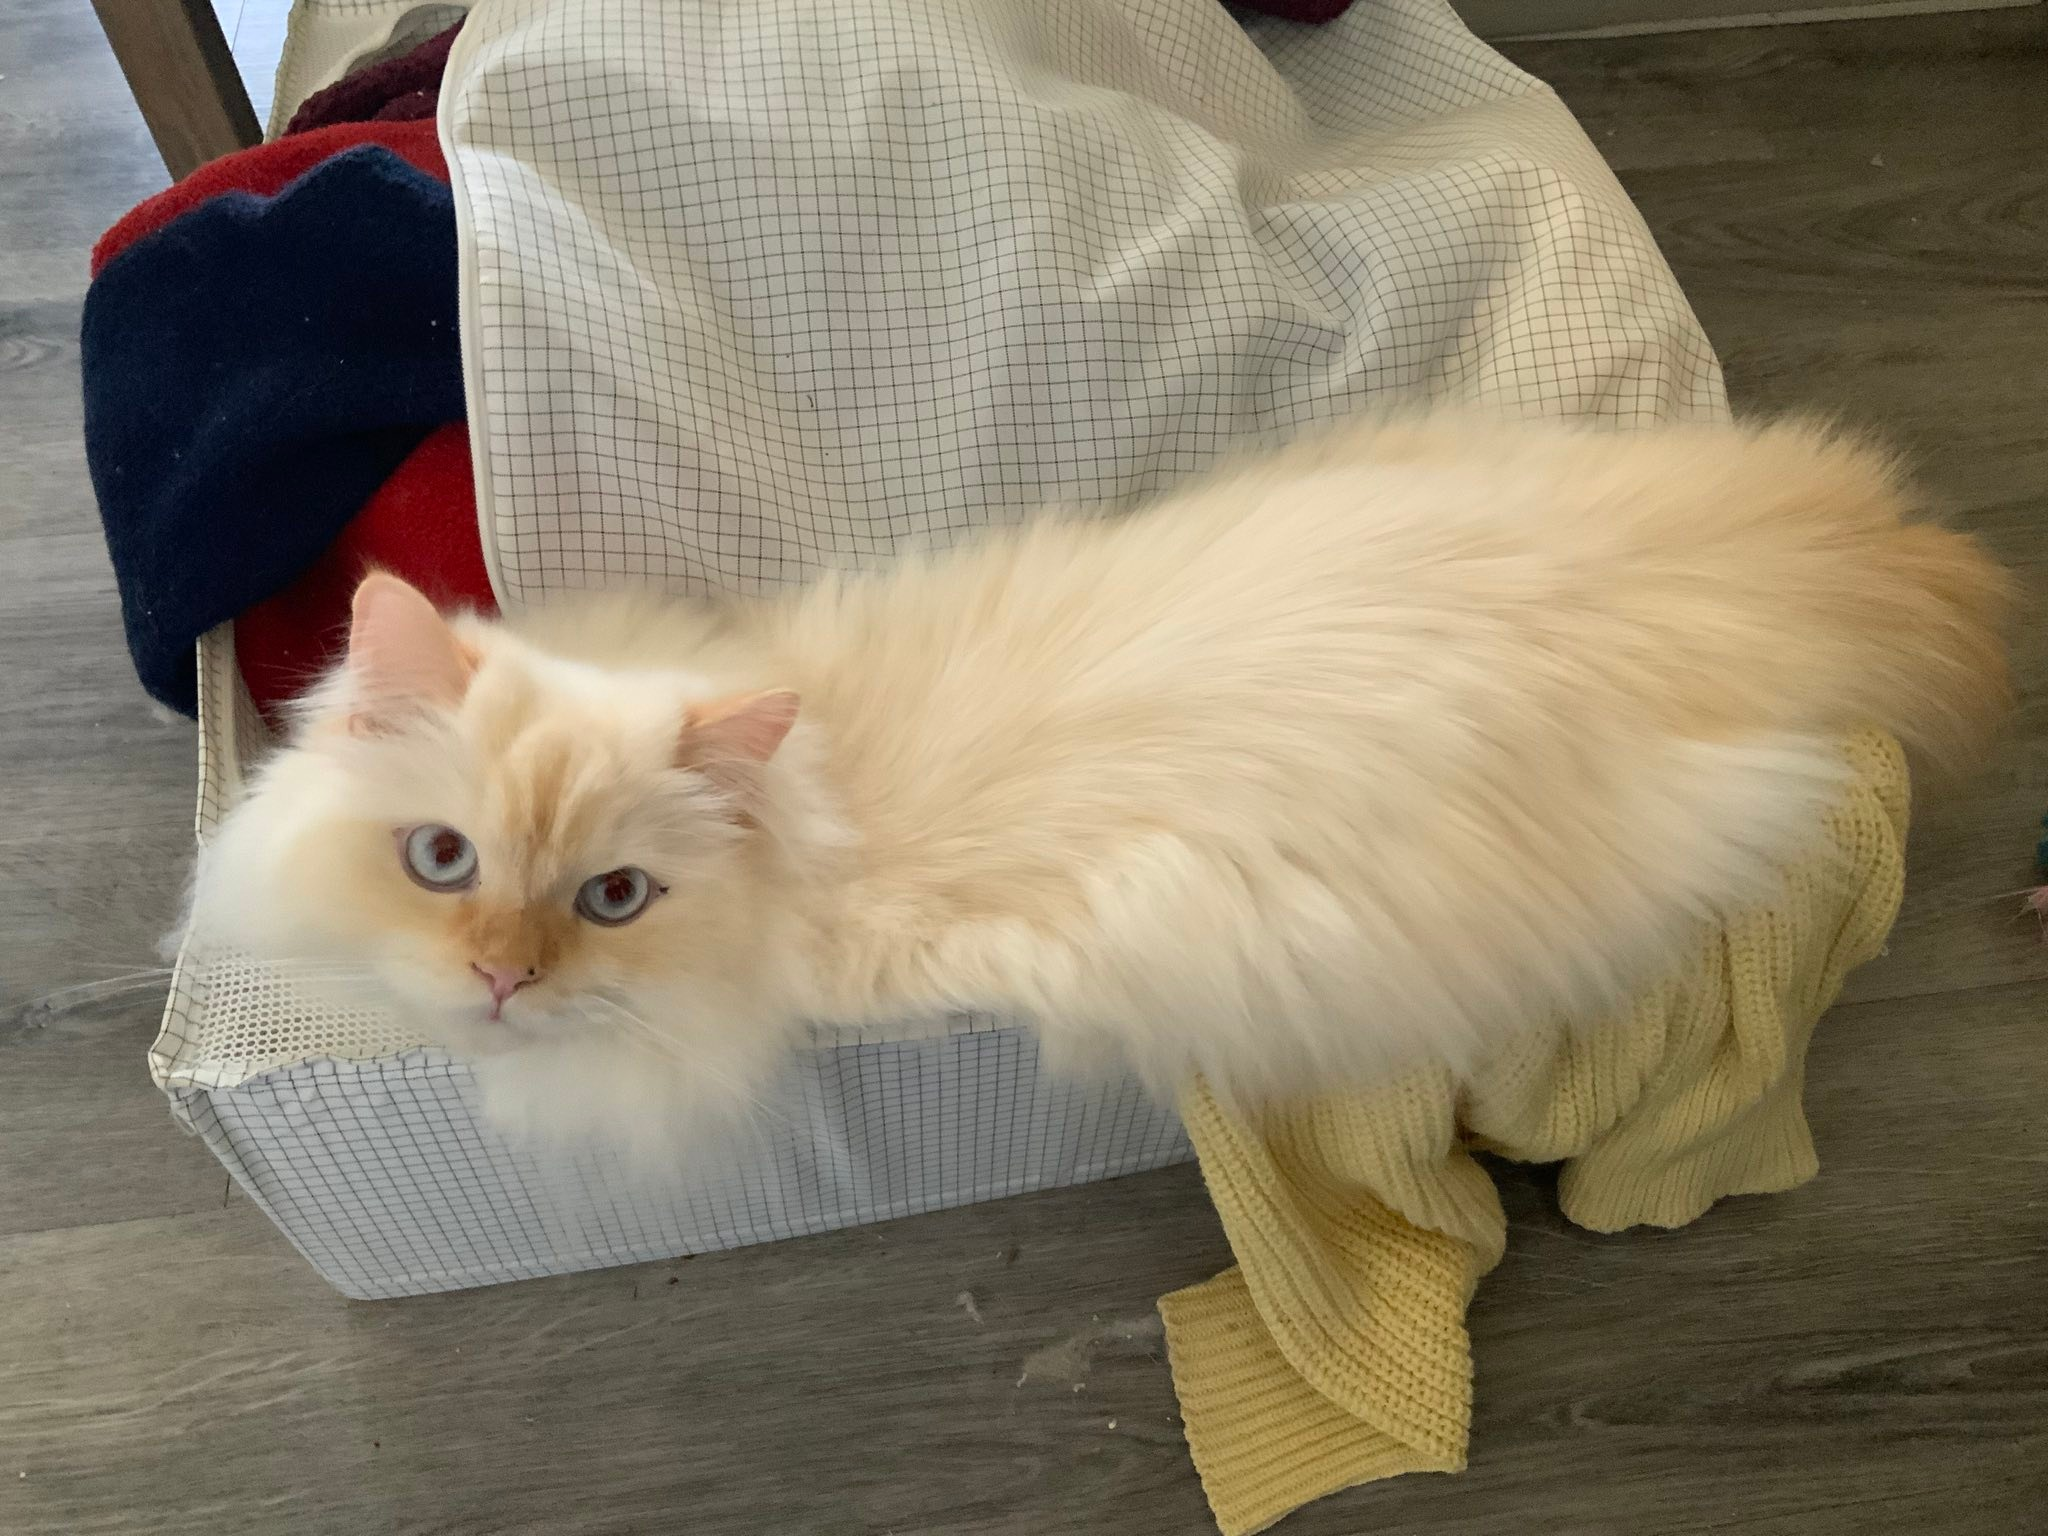
\includegraphics[height=0.3\textwidth]{davey.jpeg} & 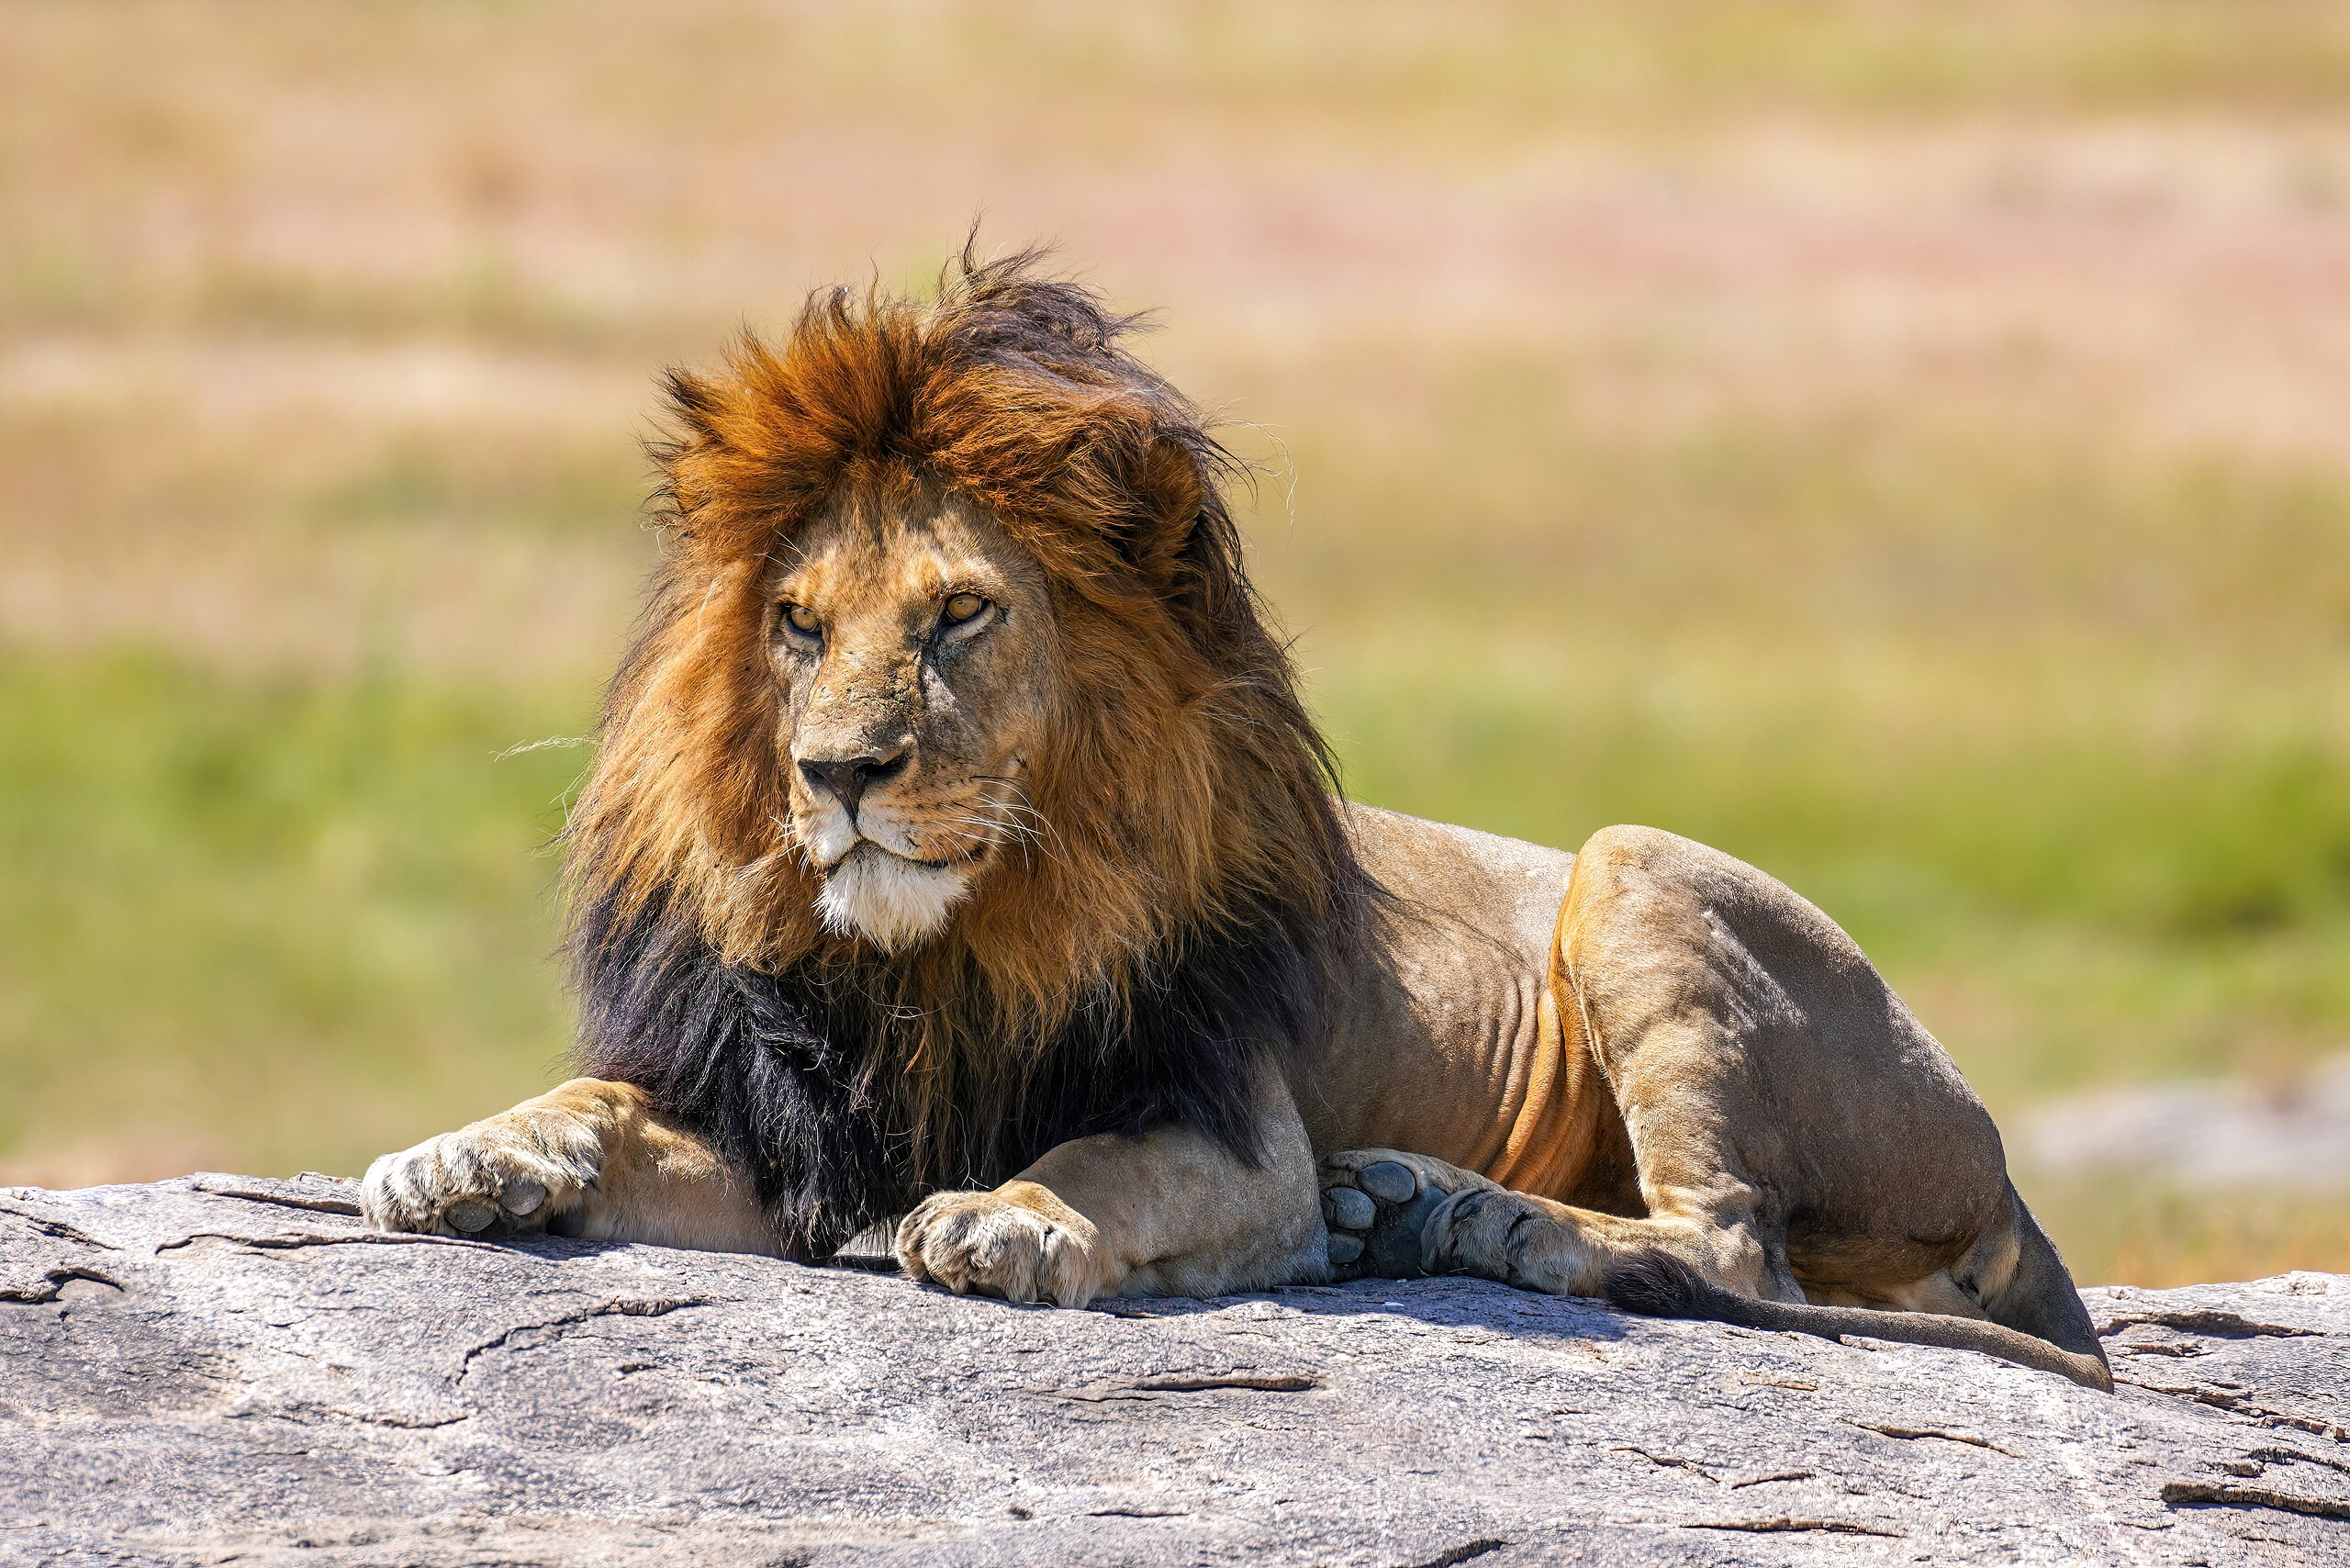
\includegraphics[height=0.3\textwidth]{lion.jpg}
        \end{tabular}
    \end{center}
\end{frame}

\begin{frame}{Ring 3}
    \begin{itemize}
        \pause \item All the code you have ever run on an x86\_64 CPU has been in ring 3.
        \pause \item Even when you're \texttt{root}, you're still in ring 3.
    \end{itemize}
\end{frame}

\begin{frame}{Ring 0}
    Much of the interesting stuff that computers do can only be done from ring 0.
    This includes
    \begin{itemize}
        \pause \item Sending/receiving data over the network
        \pause \item Reading/writing to/from files
        \pause \item Printing stuff to \textpf{stdout}
        \pause \item Interacting with peripherals
    \end{itemize}
\end{frame}

\begin{frame}{Accessing Ring 0 from Ring 3}
    \begin{itemize}
        \pause \item If all those things require ring 0 privileges, and your code runs in ring 3, how is your code able to do those things?
        \pause \item System calls!
    \end{itemize}
\end{frame}

\begin{frame}{System Calls}
    \begin{itemize}
        \pause \item System calls (a.k.a. syscalls) are how user programs ask the kernel to do privileged operations.
        \pause \item Each syscall has a unique \textit{syscall number}.
    \end{itemize}

    For example,
    \begin{itemize}
        \pause \item The \texttt{read} syscall (x86\_64 syscall number 0) reads from a file descriptor.
        \pause \item The \texttt{write} syscall (x86\_64 syscall number 1) writes to a file descriptor.
        \pause \item The \texttt{open} syscall (x86\_64 syscall number 2) acquires a file descriptor for a provided file path.
        \pause \item The \texttt{close} syscall (x86\_64 syscall number 3) closes an existing file descriptor.
        \pause \item The \texttt{exit} syscall (x86\_64 syscall number 60) exits the process.
    \end{itemize}
\end{frame}

\begin{frame}{Making a System Call}
    \begin{itemize}
        \pause \item To make a system call, use the \textpf{syscall} libc function, provided by \textpf{<unistd.h>}.
        \pause \item The first argument to this function is the syscall number of the system call you'd like to invoke.
        \pause \item The rest of the arguments depend on which system call you're invoking.
        \pause \item Consult this giant table for more details:
        \pause \item \url{https://www.chromium.org/chromium-os/developer-library/reference/linux-constants/syscalls/}
    \end{itemize}
\end{frame}

\begin{frame}{Example: Nonportable \textpf{exit}}
    \inputminted{c}{./exit_55.c}
\end{frame}

\begin{frame}{Portability}
    \begin{itemize}
        \pause \item On other OSes, and even on some other Linux machines, the \textpf{exit} syscall will have a different syscall number.
        \pause \item For this reason, it's best to use the \textpf{SYS\_*} constants defined in \textpf{<sys/syscall.h>} when possible.
    \end{itemize}
\end{frame}

\begin{frame}{Example: Portable \textpf{exit}}
    \inputminted{c}{./exit_55_portable.c}
\end{frame}

\begin{frame}{File Descriptors}
    \begin{itemize}
        \pause \item On Unix, there are 3 file descriptors that are open when a process starts:
            \begin{itemize}
                \pause \item \textpf{stdin}, file descriptor 0
                \pause \item \textpf{stdout}, file descriptor 1
                \pause \item \textpf{stderr} file descriptor 2
            \end{itemize}
        \pause \item In order to perform operations on a file, you first need to acquire a file descriptor using the \textpf{open} system call.
    \end{itemize}
\end{frame}

\begin{frame}{Activity: DIY \textpf{cat}}
    \begin{itemize}
        \pause \item Write a C program that makes a \textpf{write} system call to write something cool to \textpf{stdout}.
        \pause \item Modify your program to read $\leq 100$ bytes from \textpf{stdin}, and \textpf{write} the received data to \textpf{stdout}.
        \pause \item Modify your program to repeatedly \textpf{read} and \textpf{write} in a loop until either system call fails.
        \pause \item Make a new file called \textpf{prog\_input}. Modify your program to read from that file instead of \textpf{stdin}.
    \end{itemize}
\end{frame}

\begin{frame}{Strings}
    \begin{itemize}
        \pause \item Strings are just \textpf{char *}s.
        \pause \item Because \textpf{sizeof} doesn't work on pointers, you need some other way of knowing when a string ends.
        \pause \item One way to do this is to store strings along with their lengths.
        \pause \item Another way to do this is to designate some byte (or byte sequence) as meaning ``end of string."
        \pause \item In C, it's traditional to use the 0 byte for this purpose.
    \end{itemize}
\end{frame}

\begin{frame}{Activity: Character Count}
    \begin{itemize}
        \pause \item Write a function \textpf{unsigned long char\_count(char *s, char c)} that counts the number of occurrences of the \textpf{char} \textpf{c} in the string \textpf{s}.
        \pause \item Verify that your function works on reasonable arguments, then try passing weird arguments to your function. What does it do?
    \end{itemize}
\end{frame}

\end{document}
